\documentclass[aspectratio=1610]{beamer}

\usetheme{unnslides}

\usepackage{listings}
\usepackage{graphicx}
\usepackage{caption}
\usepackage{cmbright}
\usepackage{fontspec}
\usepackage{unicode-math}
\setmainfont{CMU Sans Serif}
\setromanfont{CMU Sans Serif}
\setsansfont{CMU Sans Serif}

\usepackage{polyglossia}
\setmainlanguage{russian}
\setbeamertemplate{itemize item}{\color{black}$\blacktriangleright$}

\graphicspath{ {../paper/images/}{img/} }
%set pages numeration
\setbeamertemplate{footline}[frame number]
\setbeamertemplate{headline}{}
\setlength\abovecaptionskip{-1pt}

\title{Исследование схем ускорения сходимости алгоритмов глобальной оптимизации}
\author{\textbf{В.В.~Соврасов}}
\institute{ННГУ им. Н.И. Лобачевского}
\date{}

\begin{document}

\begin{frame}[noframenumbering,plain]
\titlepage
\end{frame}

\begin{frame}
  \frametitle{Постановка задачи}
    \(D=\{y\in R^N:a_i\leqslant x_i\leqslant{b_i}, 1\leqslant{i}\leqslant{N}\}\) ---
    некоторый гиперинтервал, на котором определены функции задачи.
  \begin{displaymath}
    \begin{array}{c}
      Q=\{y\in D: g_j(y)\leqslant 0,  1\leqslant{j}\leqslant{m}\}  \\
      \varphi(y^*)=\min\{\varphi(y):y\in Q\}
    \end{array}
  \end{displaymath}
  Предполагается, что целевая функция \(\varphi(y)\) и ограничения \(g_j(y)\) удовлетворяет условию Липшица в области \(D\):
  \begin{displaymath}
  |\varphi(y_1)-\varphi(y_2)|\leqslant L\Vert y_1-y_2\Vert,y_1,y_2\in D,0<L<\infty
  \end{displaymath}
  Численное решение задачи означает построение оценки \(\widetilde{y}\), близкой по какой-либо
  норме к точке \(y^*\) на основе конечного числа значений целевой функции задачи,
  вычисленных в точках области \(D\).
\end{frame}

\begin{frame}
  \frametitle{Редукция размерности}
  Основные подходы:
  \begin{itemize}
    \item Использование развёрток:
    \(\lbrace y\in R^N:-2^{-1}\leqslant y_i\leqslant 2^{-1},1\leqslant i\leqslant N\rbrace=\{y(x):0\leqslant x\leqslant 1\}\),
    \(\varphi(y(x^*))=\min\{\varphi(y(x)):x\in [0;1]\}\)
    \item Многошаговая схема:
    \(\min\limits_{(x_1,..,x_n)\in D} f(x_1,..,x_n)=\min\limits_{a_1\le x_1\le b_1}\min\limits_{a_2\le x_2\le b_2}...\min\limits_{a_n\le x_n\le b_n} f(x_1,...,x_n)\)
    \item Блочная многошаговая схема:
      %
  \end{itemize}

\end{frame}

\begin{frame}
  \frametitle{Метод глобальной оптимизации}
  Общая схема характеристического метода:
  пусть имеется \(k\) результатов испытаний, далее:

  Шаг 1. Упорядочить поисковую информацию по возрастанию
  координат точек испытаний

  Шаг 2. Вычислить для каждого интервала
  величину \(R(i)\), называемую характеристикой.

  Шаг 3. Выбрать интервал номер \(t\) с наибольшей
  характеристикой и провести в нем испытание:
  \begin{displaymath}
    x^{k+1}=d(t)\in (x_{t-1}, x_t)
  \end{displaymath}

  Критерий остановки:
  \begin{displaymath}
    \Vert x_t - x_{t-1}\Vert < \varepsilon
  \end{displaymath}
\end{frame}

\begin{frame}
  \frametitle{Метод глобальной оптимизации}
  Формулы дял вычисления характеристик:

  Правила выбора следующей точки:

\end{frame}

\begin{frame}
  \frametitle{Класс тестовых задач}
  \begin{columns}
    \begin{column}{0.5\textwidth}
      Генератор GKLS:
      \begin{displaymath}
        f(x)=
      \end{displaymath}
    \end{column}
    \begin{column}{0.5\textwidth}
      \centerline{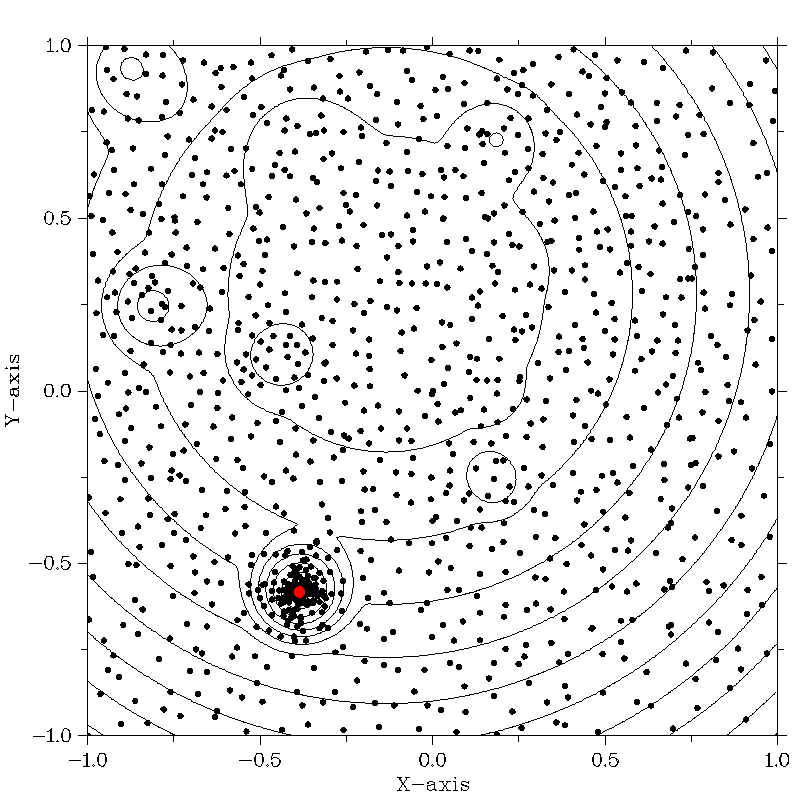
\includegraphics[width=0.9\textwidth]{gkls_loc.png}}
    \end{column}
\end{columns}
\end{frame}

\begin{frame}
\frametitle{Использование методов локальной оптимизации}
Способы использования локального поиска (метод Хука-Дживса):\
\begin{enumerate}
  \item Запуск из лучшей найденной точки после окончания работы АГП.
  \item Запуски из текущих лучших точек в процессе работы АГП.
\end{enumerate}
\bigbreak
Стратегии сохранения информации (для п. 2):
\begin{itemize}
  \item добавлять только лучшие точки
  \item добавлять в поисковую информацию все точки
\end{itemize}
\end{frame}

\begin{frame}
  \frametitle{Использование методов локальной оптимизации}
  Результаты применения различных стратегий сохранения информации:
  \begin{figure}[ht]
        \begin{minipage}[b]{0.49\linewidth}
            \centering
            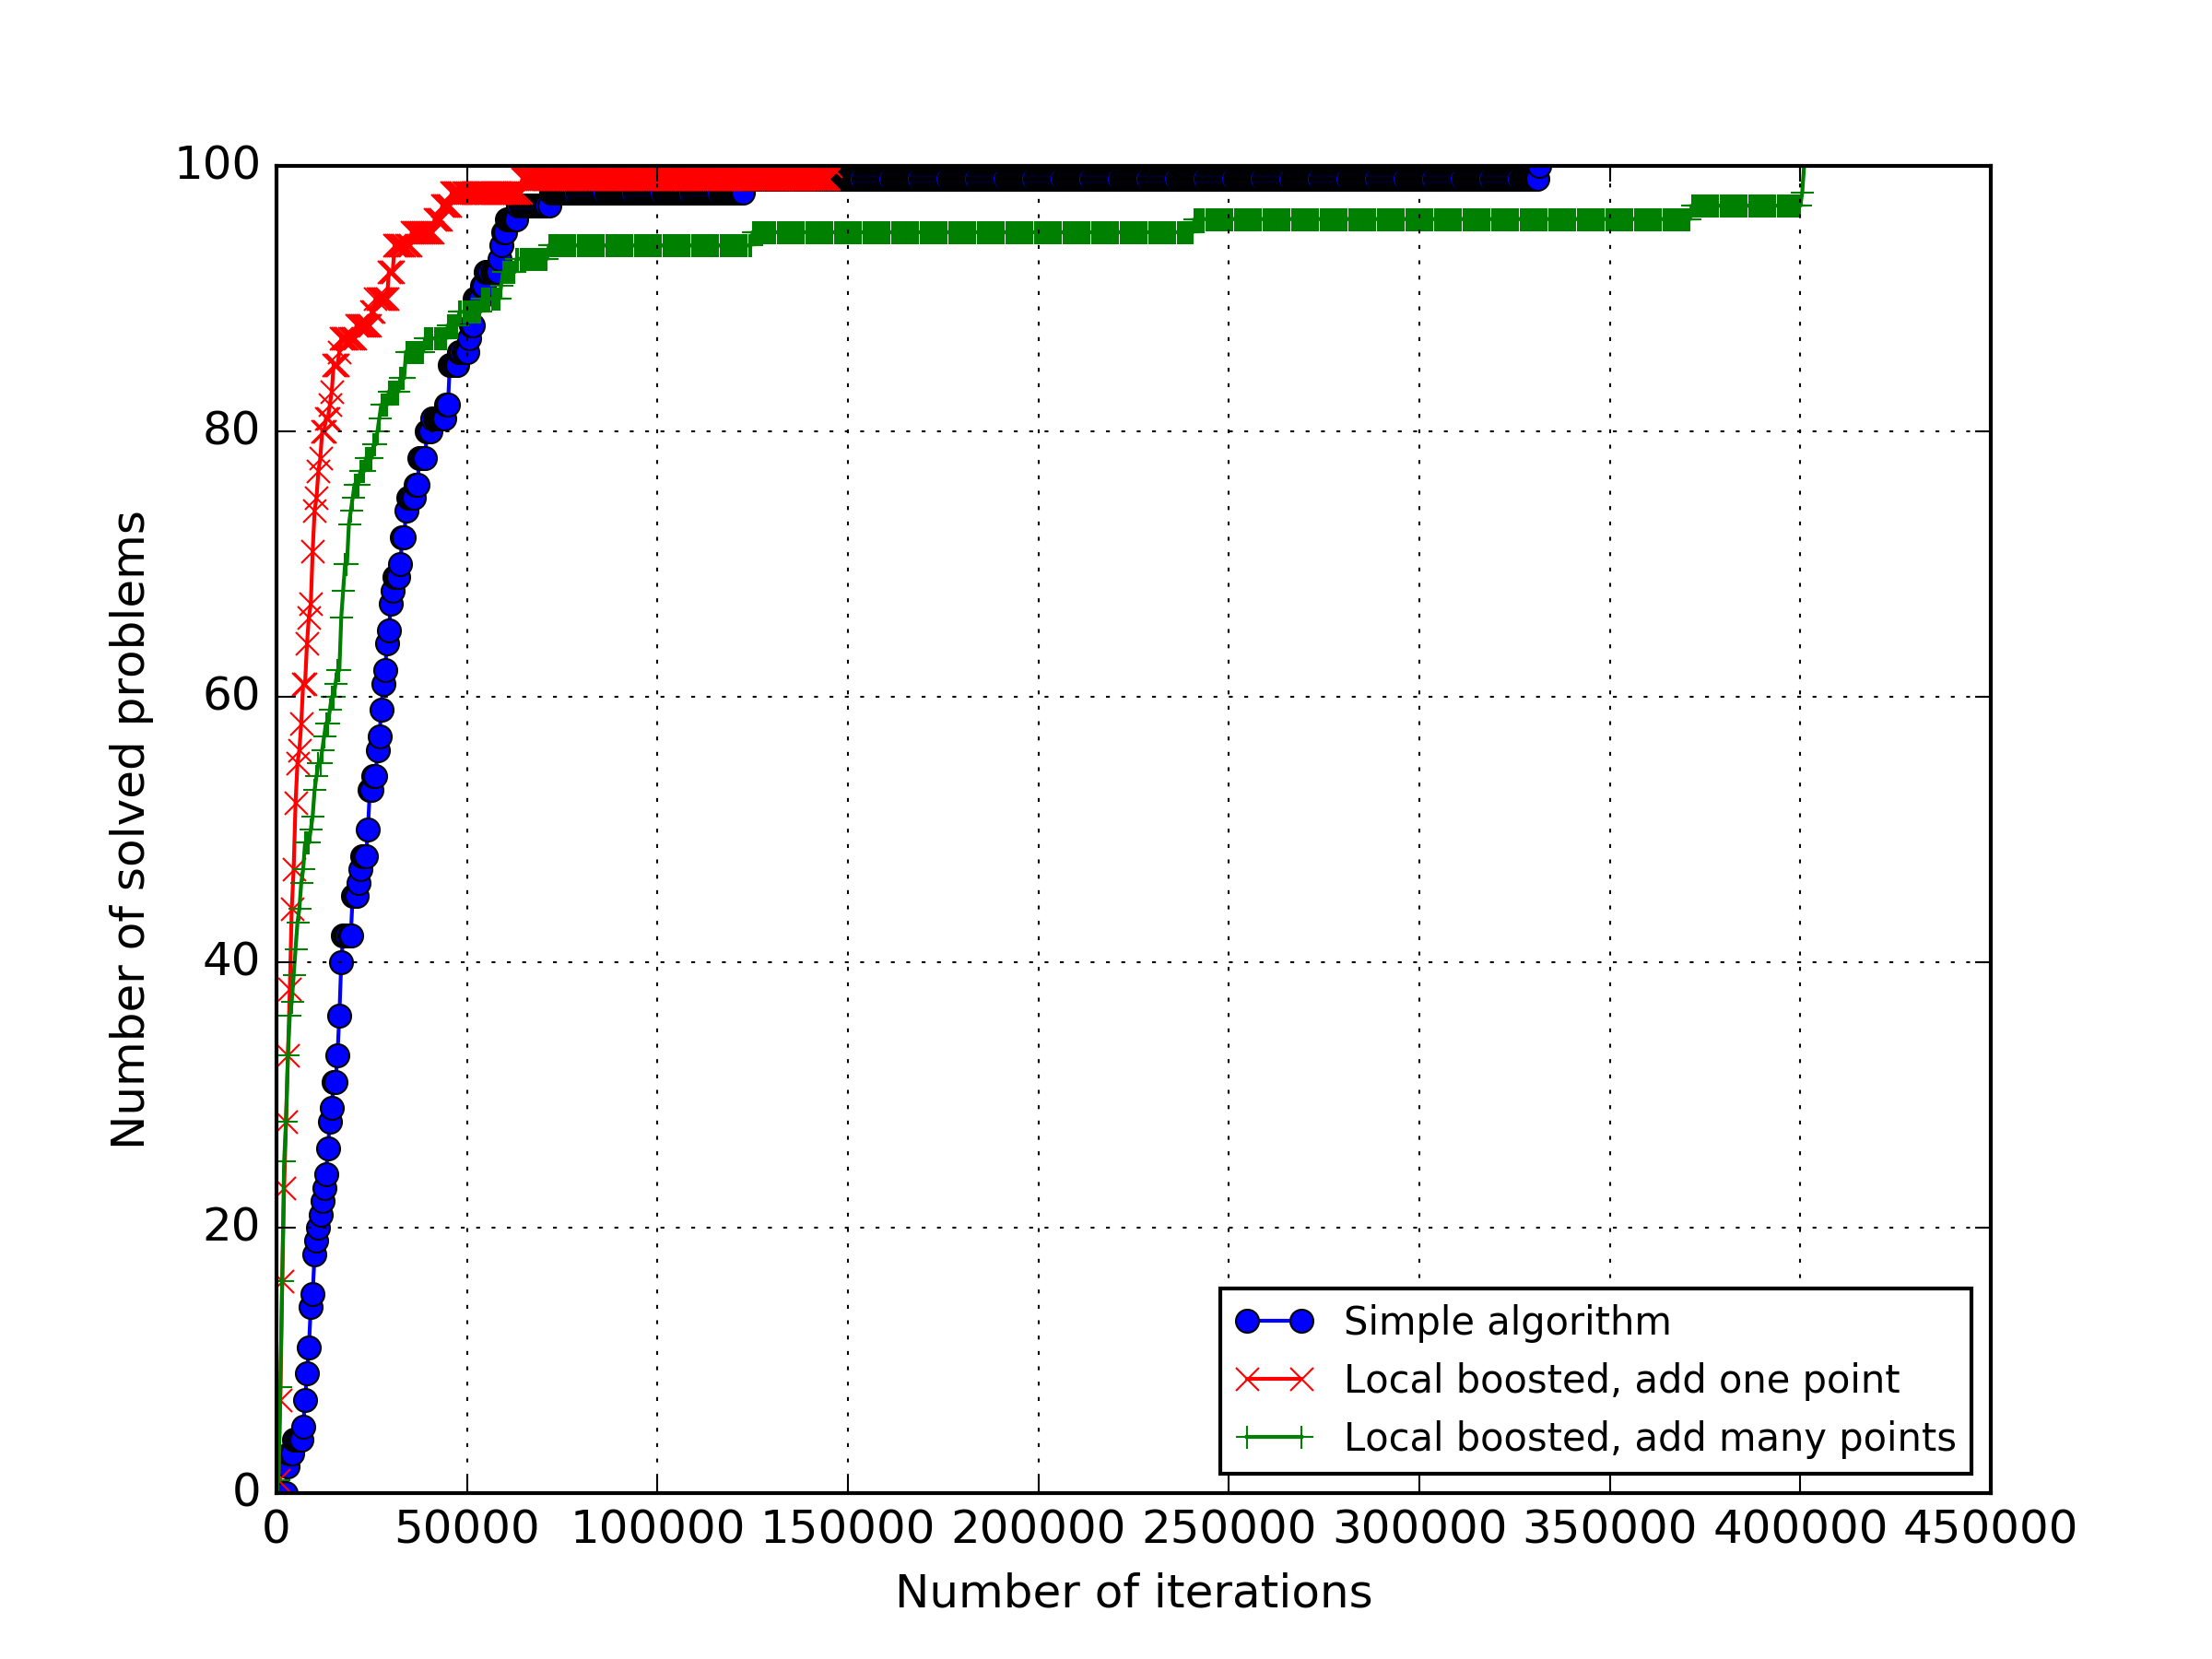
\includegraphics[width=\textwidth]{local_search_op.png}
            \caption*{GKLS 4d Simple}
        \end{minipage}
        \begin{minipage}[b]{0.49\linewidth}
            \centering
            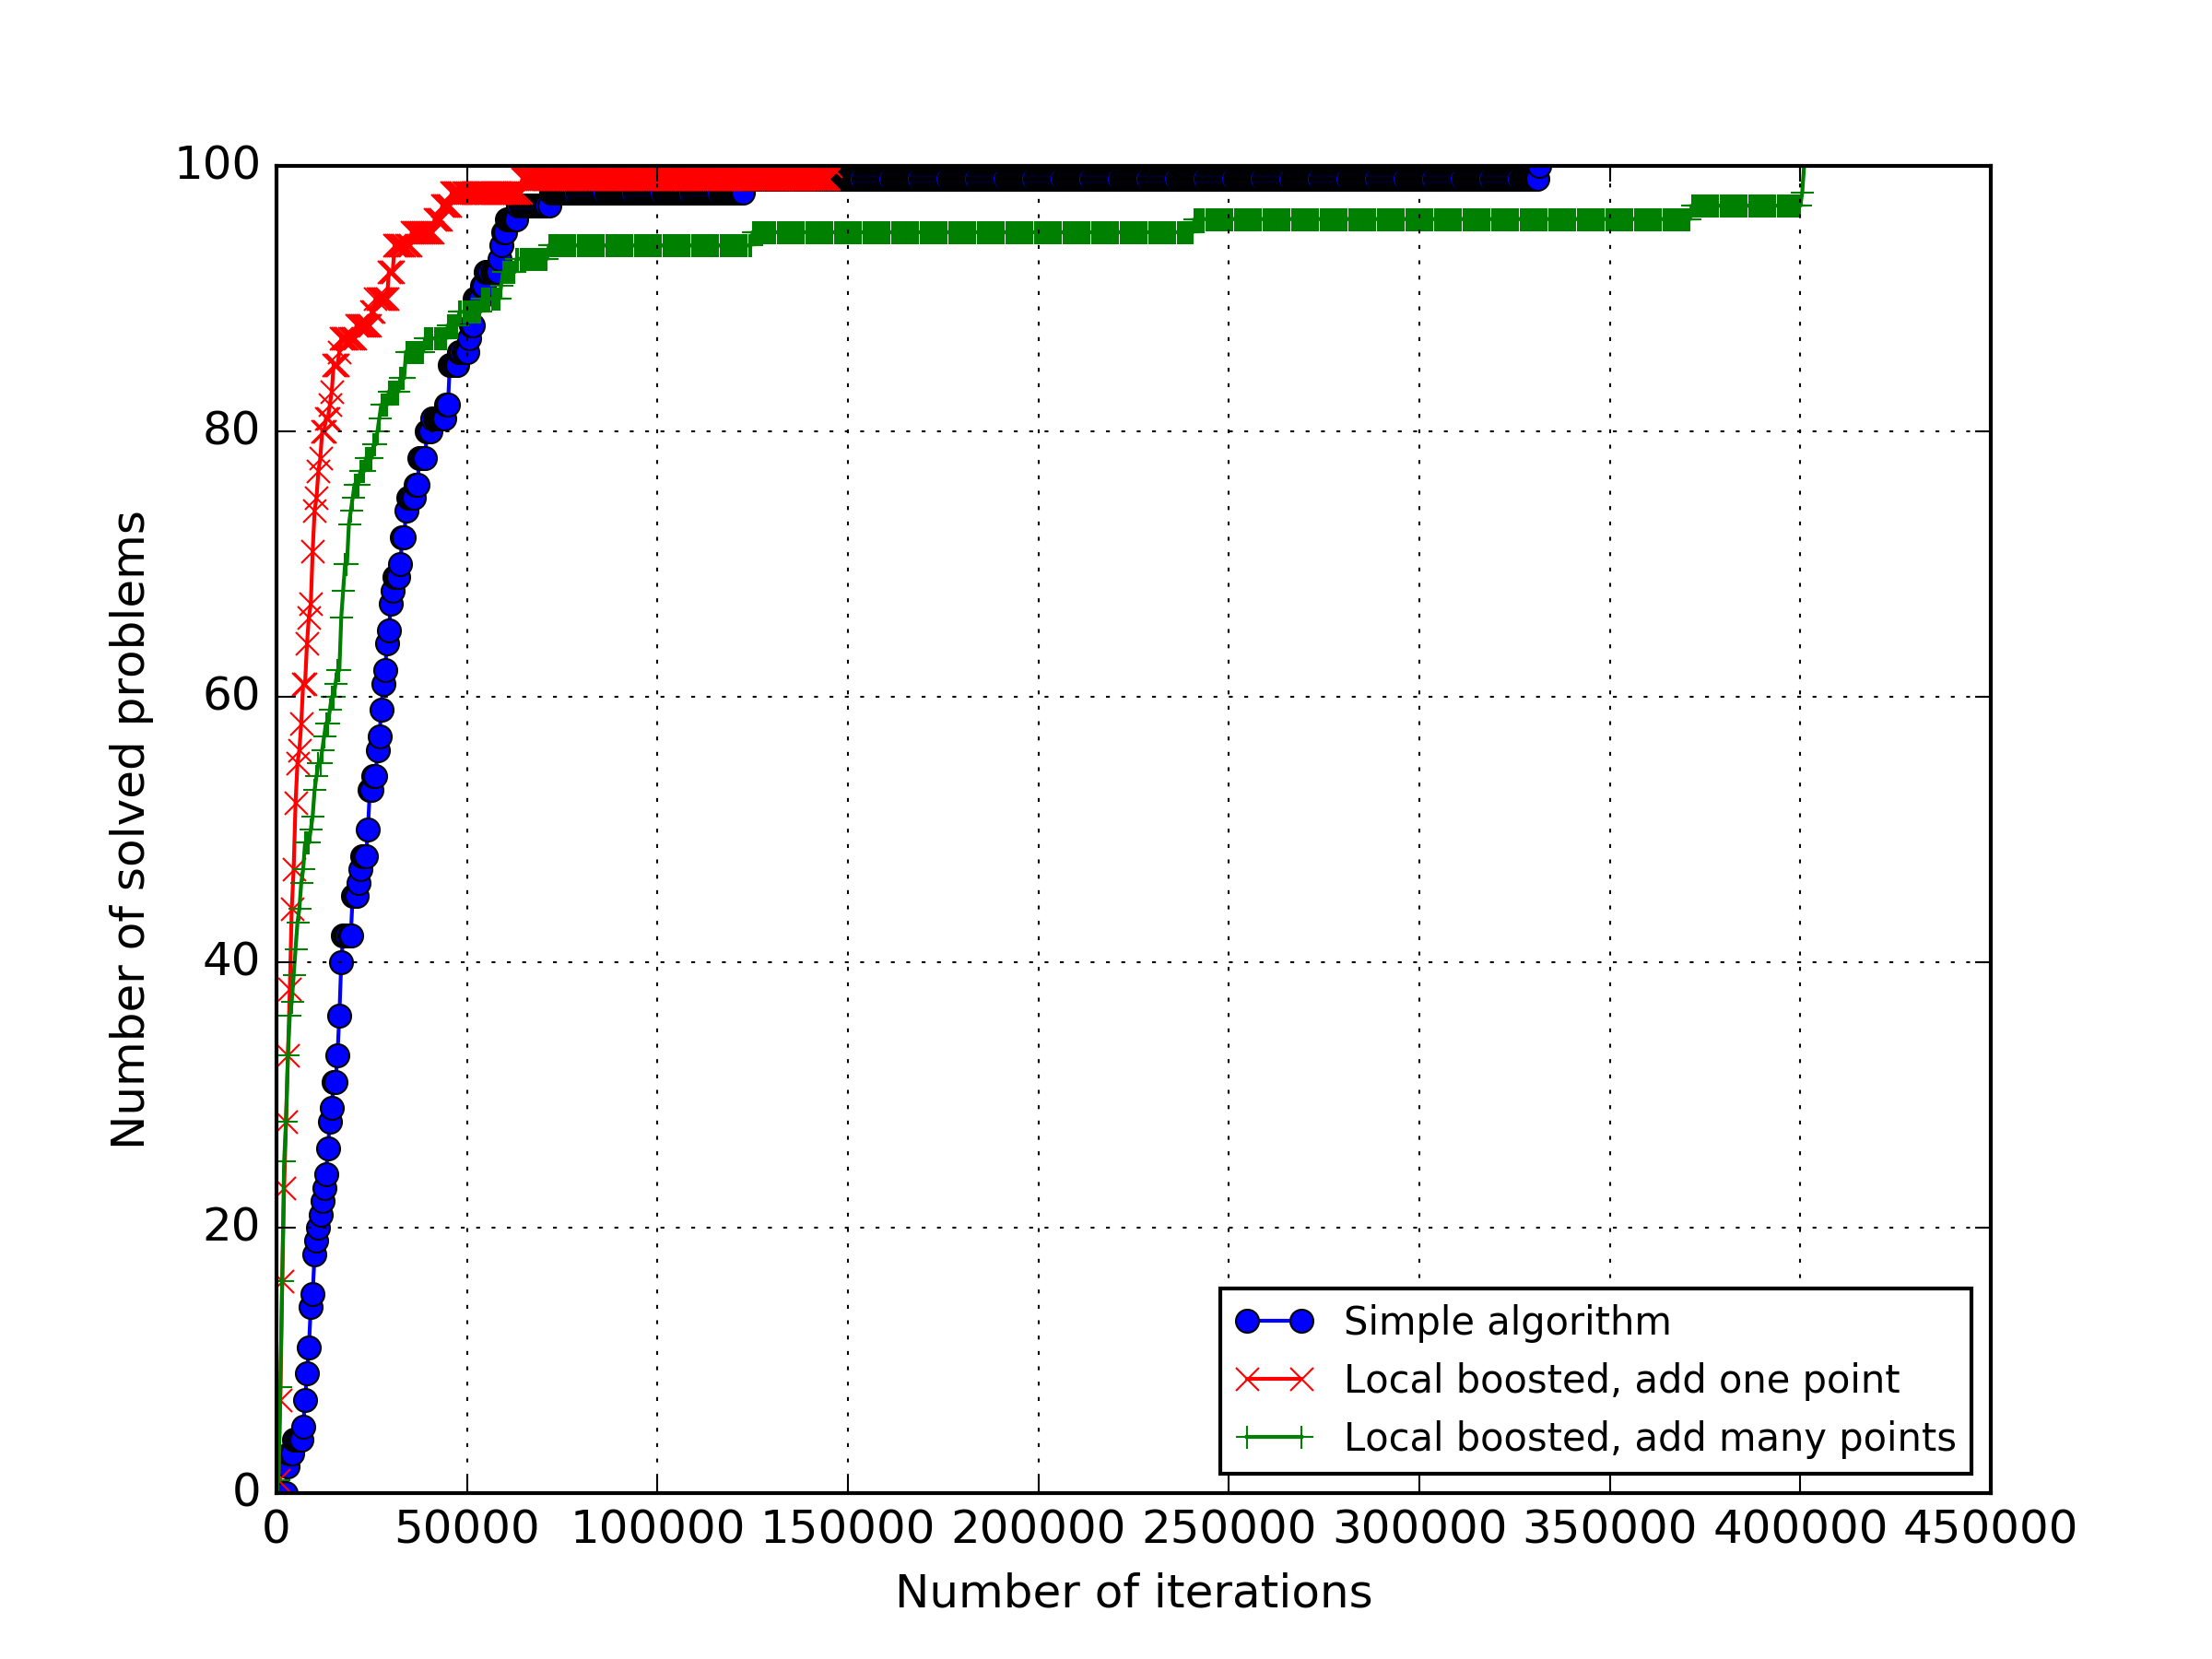
\includegraphics[width=\textwidth]{local_search_op.png}
            \caption*{GKLS 5d Simple}
        \end{minipage}
    \end{figure}
\end{frame}

\begin{frame}
\frametitle{Смешанный алгоритм}
Метод является модификацией АГП. Каждый интервал имеет две
характеристики \(R(i)\) и \(R^*(i)\).
  \begin{displaymath}
  R^*(i)=\frac{R(i)}{\sqrt{(z_i-z^*)(z_{i-1}-z^*)}/\mu + 1.5^{-\alpha}}
  \end{displaymath}
  Для эффективной реализации АГП используется приоритетная
  очередь интрервалов. Ключ – \(R(i)\).
  Для смешанного АГП – две связанные очереди.
  Операции с очередями:
  \begin{itemize}
    \item Синхронная вставка
    \item Синхронное удаление
    \item Обновление перекрестных ссылок при восстановлении кучеобразности
  \end{itemize}
\end{frame}

\defverbatim[colored]\lstI{
\begin{lstlisting}[language=C++,keywordstyle=\color{red}]
inline void swapElems(T& arg1, T& arg2)
{
  if (arg1.pLinkedElement != NULL &&
      arg2.pLinkedElement != NULL)
    std::swap(arg1.pLinkedElement->pLinkedElement,
      arg2.pLinkedElement->pLinkedElement);
  else if (arg1.pLinkedElement != NULL)
    arg1.pLinkedElement->pLinkedElement = &arg2;
  else if(arg2.pLinkedElement != NULL)
    arg2.pLinkedElement->pLinkedElement = &arg1;
  std::swap(arg1, arg2);
}
\end{lstlisting}
}

\begin{frame}
\frametitle{Смешанный алгоритм}
Схема перекрёстных ссылок на элементы очередей:
    \begin{figure}
      \center
        \includegraphics[width=.7\textwidth]{examin_heaps.png}
    \end{figure}
\end{frame}

\begin{frame}
\frametitle{Смешанный алгоритм}
Алгоритм обмена элементов при погружении/всплытии:
\lstI
\end{frame}

\begin{frame}
  \frametitle{Смешанный алгоритм}
  \begin{figure}
    \center
      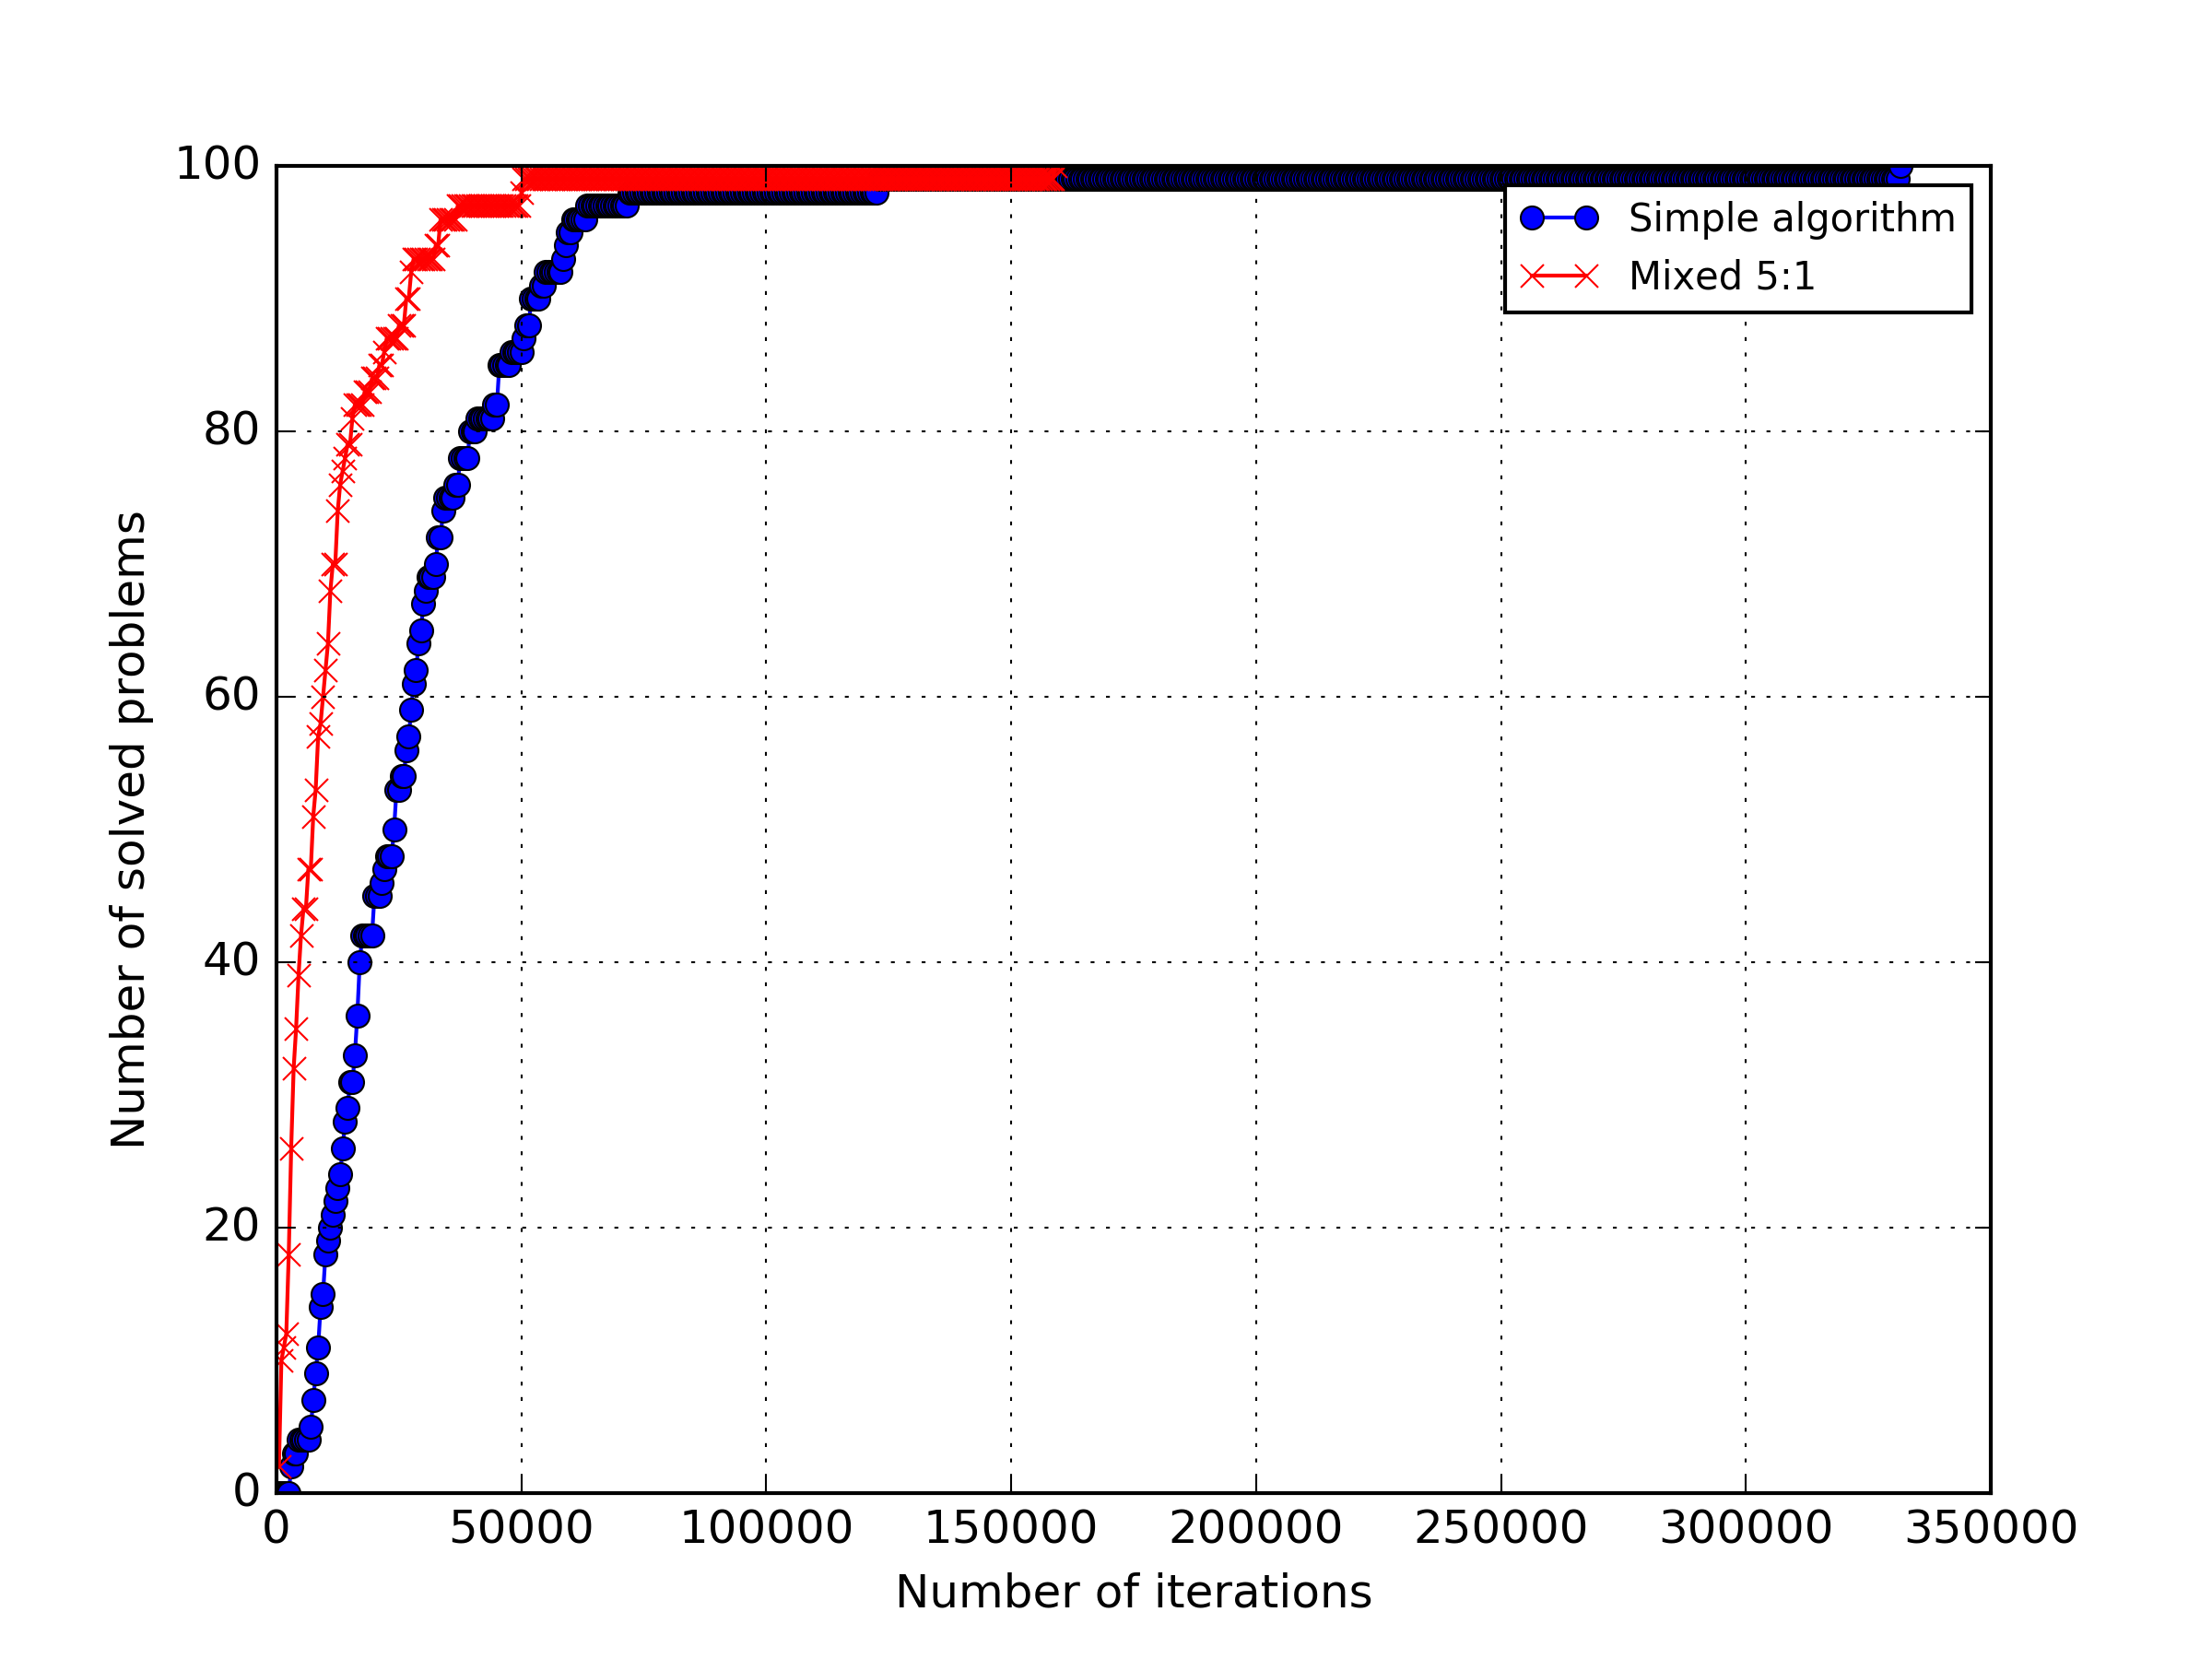
\includegraphics[width=0.7\textwidth]{mixed_op4d.png}
      \caption*{Операционные характеристики обычного и смешанного АГП на классе GKLS 4d Simple}
  \end{figure}
\end{frame}

\end{document}
